General Explanation of the plots:
\begin{center}
    \begin{tabular}{ l c l }
%        \toprule
        \textbf{Element} & & \textbf{Meaning} \\
        \midrule\midrule
        blue background & & goal classifier \\
        \midrule
        green and red points & & example nodes labeled 1 and 0 respectively \\
        \midrule
        x markers & & test examples we discussing \\
        \midrule
        red lines & & goal classifier returns 0 \\
        \midrule
        blue lines & & goal classifier returns 1 \\
%        \bottomrule
    \end{tabular}
\end{center}


\subsection{}
With reference to Fig. \ref{Q2_a}, ID3 algorithm will discard feature $v_1$ and keep only feature $v_2$ (achieving the goal classifier) by setting $v_{2}>0$ for class 1, while KNN, given that the two points are equidistant, will return the class of the one with higher $v_2$ value, which is wrong.

\begin{figure}[H]
    \centering
    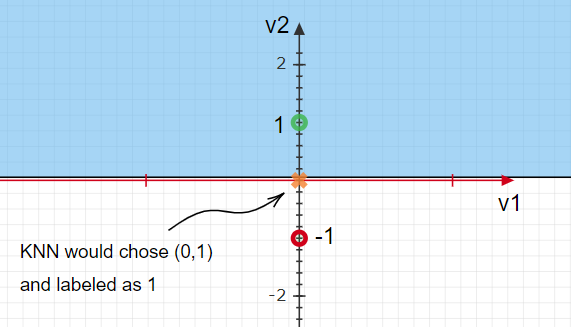
\includegraphics[width=0.6\linewidth]{a.png}
    \caption{Training set: $D=\{<(0,1),1>,<(0,-1),0>\}$. Goal classifier $F_{true}=1\ \text{if}\ v_{2}>0$. ID3: $v_{2}>0$ (goal classifier). KNN: $x_{q}=(0,0)$; $d(x_{q},(0,1))=d(x_{q},(0,-1))$; $KNN(x_{q})=1$; $\exists x_{q}:\ KNN(x_{q})\neq F_{true}$.}
    \label{Q2_a}
\end{figure}


\subsection{}
With reference to Fig. \ref{Q2_b}, KNN will always be right, also on the dividing line, consistently with the goal classifier. ID3 will chose feature $v_1$ and discard feature $v_2$ because the leaves are reached after one decision node and no more splitting is available while building th tree.

\begin{figure}[H]
    \centering
    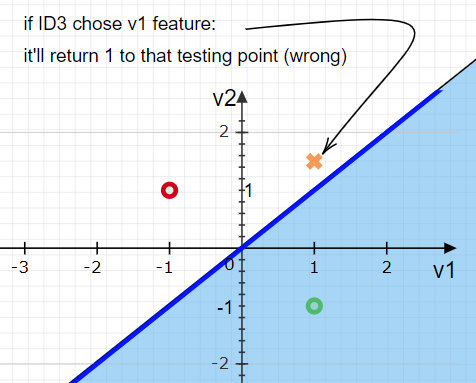
\includegraphics[width=0.5\linewidth]{b.png}
    \caption{Training set: $D=\{<(1,-1),1>,<(-1,1),0>\}$. Goal classifier: $F_{true}=\begin{cases} 1\ v1\geq v2\\ 0\ v1<v2 \end{cases}$.\\ KNN: achieves the goal classifier. ID3: only uses one feature and does not achieve the goal classifier.}
    \label{Q2_b}
\end{figure}

%The ID3 will use only one feature cause after one division it riches
%a leaf e.g. taking $v1>0\ or\ v2>0$ and this is clearly bad. (see
%image)
%
%KNN will be right in every situation. if $x_{q}$features are equal
%$v_{1}=v_{2}$ , the distances to both training nodes are equal and
%it will take the positive nodes $<(1,-1),1>$ because of higher $v_{1}$
%which is consistent with the true classifier. Else $x_{q}:v_{1}\neq v_{2}$
%it will classify right by computing the distances to the nearest example
%node.


\subsection{}
With reference to Fig. \ref{Q2_c}, given $K=1$, ID3 will only use one feature, because it reaches the leaves after defining the first decision node, achieving a bad classifier. KNN will also achieve a bad classifier for points on the line $v_{1}=v_{2}$, as already seen in the answer to question A.

\begin{figure}[H]
    \centering
    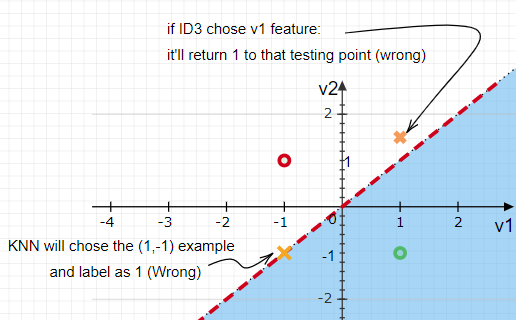
\includegraphics[width=0.6\linewidth]{c.png}
    \caption{$K=1$. Training set: $D=\{<(1,-1),1>,<(-1,1),0>\}$. Goal classifier: $F_{true}=\begin{cases}1\ v1>v2\\0\ v1\leq v2\end{cases}$.\\ KNN: $v_{1}=v_{2}$. ID3: $v1>0\ or\ v2>0$.}
    \label{Q2_c}
\end{figure}

%KNN will be wrong at points whose : the distances to
%both training nodes are equal and it will take the positive nodes
%$<(1,-1),1>$ because of higher $v_{1}$ and return True (1).
%
%However the true classifier will label it as False (0).

\subsection{}
With reference to Fig. \ref{Q2_d}, given $K=1$, ID3 will split according to $v_2\geq0$ feature only and thus reach the leaves of the decision tree; KNN will compute the distance from the training data, and points on the limiting line will be assigned label 1 because the label of the xample with the higher $v_2$ value is returned, thus agreeing with the goal classifier.

\begin{figure}[H]
    \centering
    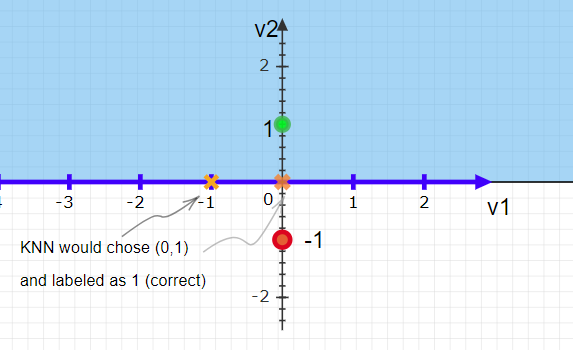
\includegraphics[width=0.6\linewidth]{d.png}
    \caption{$K=1$. Training set: $D=\{<(0,1),1>,<(0,-1),0>\}$. Goal classifier: $F_{true}=1\ if\ v_{2}\geq0$.\\ KNN: $v_{2}\geq0$. ID3: $v_{2}\geq0$.}
    \label{Q2_d}
\end{figure}


%ID3: $v_{1}$ feature isn't informative and by using $v_{2}$ we can get to the leaves. ID3 will check if $v_{2}>0$ and we will get the goal classifier.
%
%KNN: if $x_{q}:v2=0$, the distance to the examples are equal and the label will be taken from the higher $v_{2}$ example and return 1 (Right). else ($v_{2}\neq0)$ the KNN is working good. for $v_{2}>0$ the nearest example is (0,1) and the label is 1 and for $v_{1}<0$ the nearest example is (0,-1) and the label is 0, thus in both cases it is consistent with classifier).
%
%Thus \textbf{KNN and ID3 are always right}
